\documentclass[11pt]{article}
%\renewcommand{\thesection}{\Roman{section}}  %zmiana section na rzymskie
\usepackage[utf8]{inputenc}
\usepackage[OT4]{polski}
\usepackage{tabularx}
\usepackage[margin=60pt]{geometry}
\usepackage{amsmath}
\usepackage{amsfonts}
\usepackage{listings} 
\usepackage[usenames,dvipsnames,table,xcdraw]{xcolor}
\usepackage{array}
\usepackage{sidecap} %do grafik
\usepackage{wrapfig} % j. w.
\usepackage{graphicx} %j.. w.
\usepackage{subfig} %j. w.
\usepackage{booktabs}
\usepackage{longtable}
\usepackage{hyperref}
\usepackage{nicefrac}
\usepackage{multirow}



\title{B.2 Środek ciężkość i moment bezwładności sześcianu.}
\author{Paweł Rzońca}

\begin{document}

\maketitle

\section*{Wstęp}

Ćwiczenie polega na wyznaczeniu środka ciężkości oraz momentu bezwładności sześcianu względem osi przechodzącej przez
jego środek i równoległej do jednego z boków. Rozważamy sześcian jednorodny o gęstości $\rho (\vec{r})=1$. 
Do wyznaczenia odpowiednich całek, użyto metody Monte Carlo.

W metodzie Monte Carlo korzystamy z twierdzenia o wartości średniej i całkę szacujemy wzorem
\begin{equation}
	I_N =\Omega \left< f \right> =  \frac{\Omega}{N}\sum_{i/0}^{N-1} f(\vec{x_i})
\end{equation}
Gdzie $\Omega$ jest objętością obszaru całkowania, a $N$ liczbą losowań. 

Środek ciężkości wynika w oczywisty sposób z symetrii figury. Przyjmując układ współrzędnych zaczepiony w połowie głównej przekątnej
sześcianu, środek układu współrzędnych pokrywa się ze środkiem ciężkości rozważanej bryły, tj. 
\begin{equation}
r_{cm}=(0,0,0).
\end{equation} 
Moment bezwładności jednorodnego sześcianu względem dowolnej osi przechodzącej przez jego środek, co można łatwo udowodnić analitycznie
, wynosi 
\begin{equation}
I = 1/6.
\end{equation}

\section*{Wyniki}
\subsection*{(a)}
Obliczono środek ciężkości oraz moment bezwładności względem osi przechodzącej przez środek 
zadanego sześcianu przyjmując środek układu współrzędnych jako środek przekątnej sześcianu. Otrzymane wyniki 
w metodzie Monte Carlo oraz wyniki analityczne przedstawiono na wykresach \ref{fig:11} i \ref{fig:22}. 
Moment bezwładności dla każdej osi przechodzącej przez środek sześcianu wynosi $1/6$. Na wykresie przedstawiono
wyniki dla trzech prostych wybranych przypadkowo.

\begin{figure} 
\centering
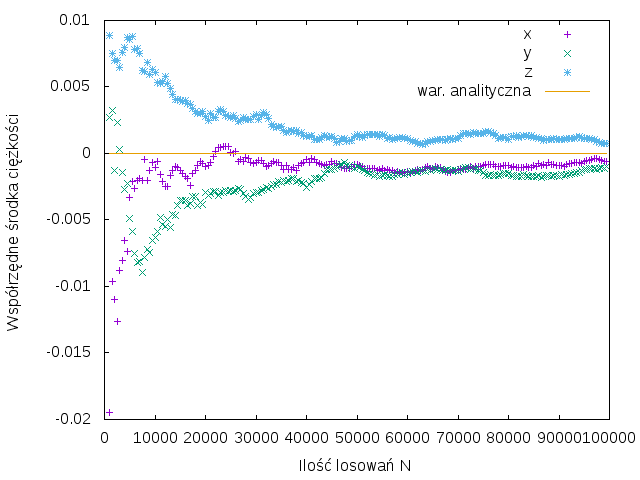
\includegraphics[width=0.7\textwidth]{CM1.png}
\caption{Obliczone współrzędne środka ciężkości w zależności od liczby losowań $N$.}\label{fig:11}
\end{figure}
\begin{figure} 
\centering
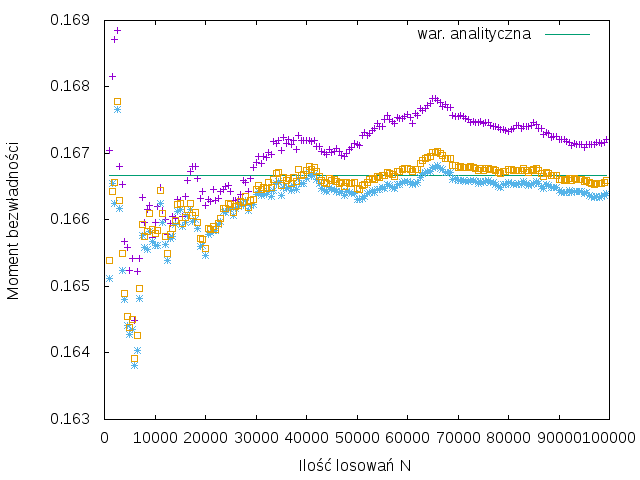
\includegraphics[width=0.7\textwidth]{EI.png}
\caption{Obliczony moment bezwładności w zależności od liczby losowań $N$ dla trzech osi przechodzących 
przez środek sześcianu.}\label{fig:22}
\end{figure}
\subsection*{(b)}
Narysowano wykres błędu $\epsilon = | I_{num} - I_{analotyczne} |$ 
w funkcji $N$ (Rys. \ref{fig:1}, zaznaczono linię dla błędu równego 0.001).
\begin{figure} 
\centering
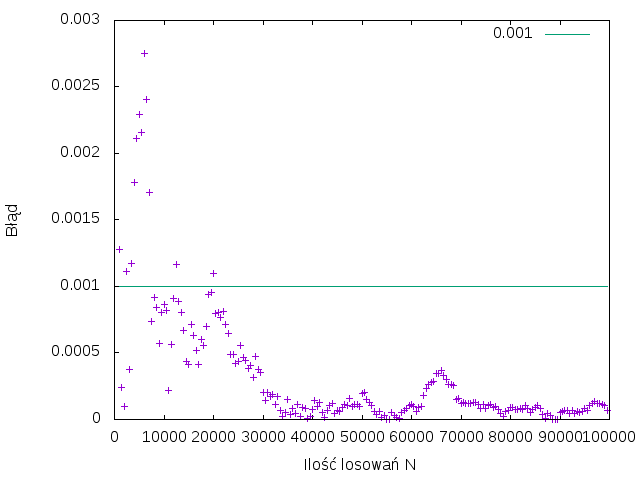
\includegraphics[width=0.7\textwidth]{ERR3.png}
\caption{Wykres błędu momentu bezwładności obliczonego metodą Monte Carlo.}\label{fig:1}
\end{figure}
\subsection*{(c)}
Moment bezwładności obliczono $M=10000$ razy i dla każdego przypadku wyznaczono błąd $\epsilon$. Uśredniony 
błąd przedstawiono na wykresie \ref{fig:2}.
\begin{figure} 
\centering
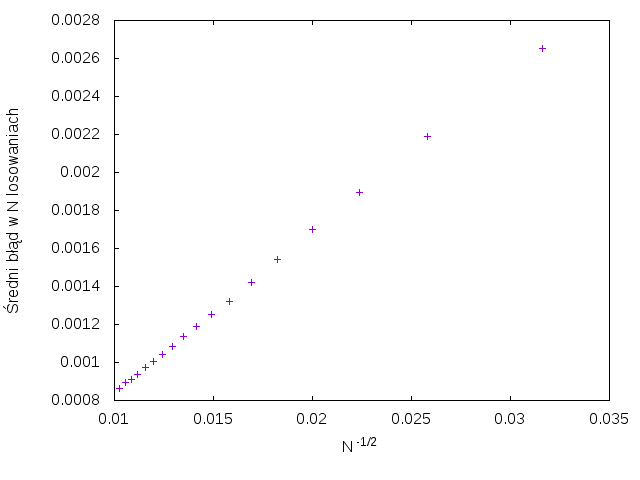
\includegraphics[width=0.7\textwidth]{ERR5.png}
\caption{Średni błąd uzyskany przy 10 tysiącach powtórzeń obliczania momentu bezwładności metodą Monte Carlo.}\label{fig:2}
\end{figure}
\section*{Podsumowanie}
Obliczone współrzędne środka ciężkości oraz moment bezwładności obliczone w ćwiczeniu metodą Monte Carlo już stosunkowo dla
małych $N$ są bardzo bliskie wynikom analitycznym. Moment bezwładności obliczono dla kilku osi przechodzących przez środek
sześcianu wybranych w sposób przypadkowy. 
Sprawdzono, że średni błąd otrzymany w metodzie Monte Carlo jest proporcjonalny do $N^{-1/2}$.  


\begin{thebibliography}{9}
\bibitem{11}
    \url{http://www.ftj.agh.edu.pl/~adamowski/wyklady_mofit_1/r3.pdf}
\end{thebibliography}



\end{document}


